\documentclass[main.tex]{subfiles}

\begin{document}
        \chapter{L'efficience des marchés du travail} 
        \emph{Est ce que le marché du travail tel qu'on le conçoit est efficace pour mettre en place la meilleure allocation de la main d'oeuvre?}

        \section{Quelle norme pour le taux de chômage}

        \begin{minipage}{0.5\textwidth}
                La courbe de Philips montre que le taux de chômage est étroitement lié au taux d'inflation, on parle de NAIRU, \emph{Non Accelerating Inflation Rate Unemployment}. La courbe de Philips calcul un taux de chômage idéal compatible avec un taux d'inflation stable. Cette donnée est utile si la courbe est validé.         \end{minipage}
        \hfill
        \begin{minipage}{0.5\textwidth}
                \center
                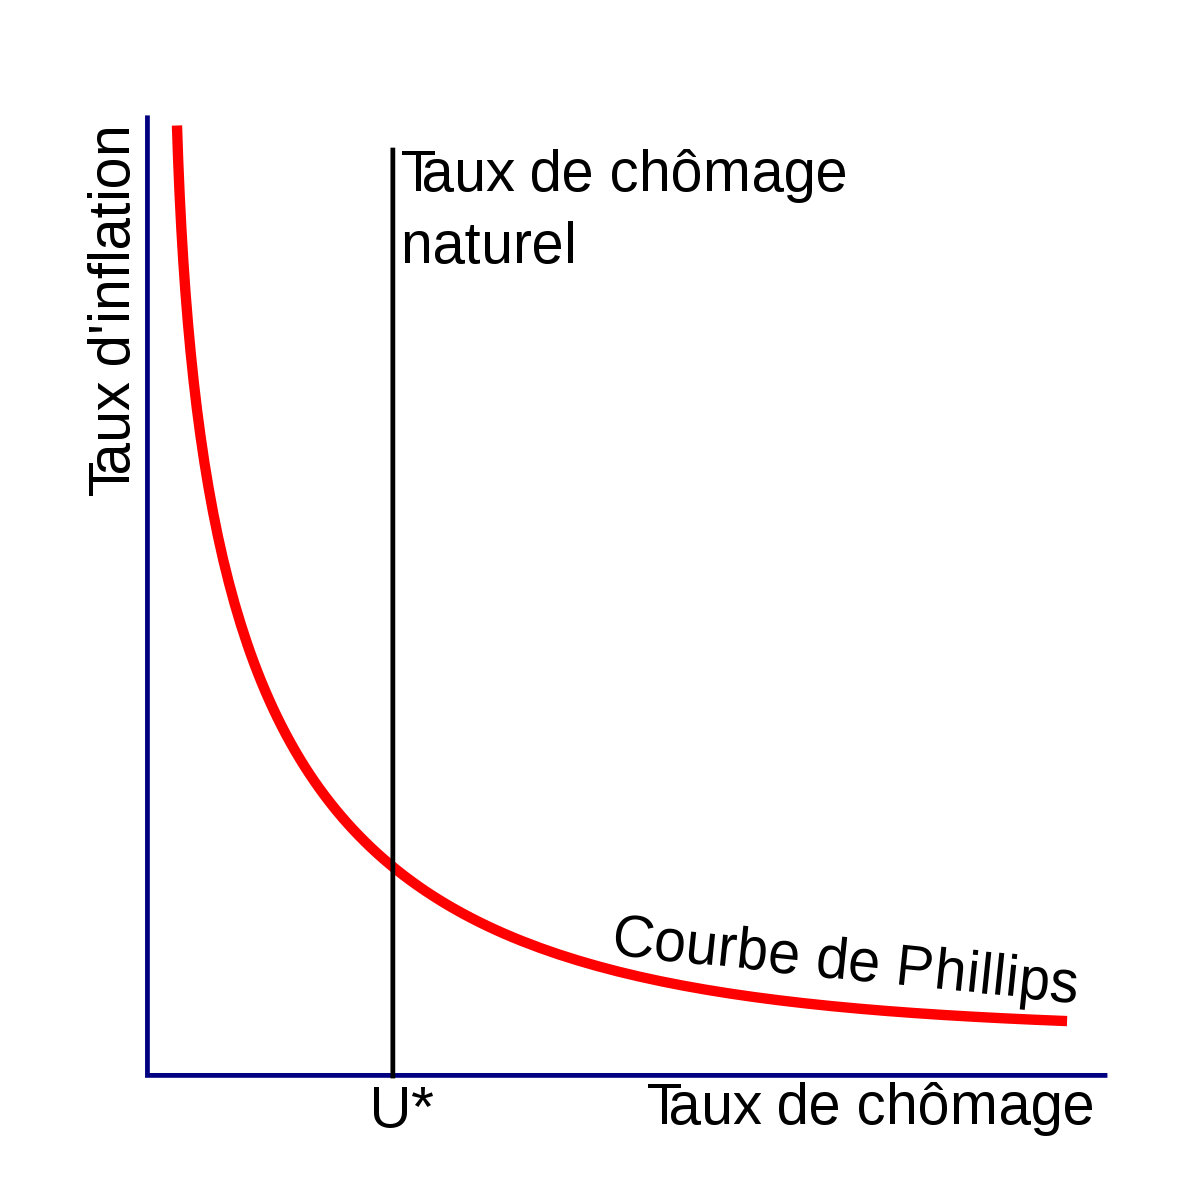
\includegraphics[width=0.8\textwidth]{nairu.png}
        \end{minipage}
        \medskip

On considère aussi le taux de chômage naturel, \emph{Natural rate of Unemployment}. Pour un niveau de compétence donné, il découle du refus des travailleurs d'accepter un salaire jugé trop faible, concept de chômage volontaire et de salaire de réserve, et du manque d'intérêt pour les firmes à proposer un salaire trop élevé. \\

Enfin on considère le taux de croissance minimal pour générer de l'emploi, ce dernier depend de la productivité et de la population active mais aussi des politiques de l'emploi avec par exemples la politique des \emph{`mini job'} en Allemagne. Cette politique vise à inonder le marché du travail de personnes peu qualifiées pour des emplois d'appoints. Les \emph{`mini job'} sont des contrats à temps partiel, faisant naturellement chuter le chômage et avec lui le taux de croissance à partir duquel le chômage baisse, mais aussi la productivité du pays.
\medskip

\begin{center}
        \begin{tabular}{|*{3}{c|}}
               \hline
               & 1970 & 2007 \\
               \hline
               Taux de croissance minimal & 2,6\% & 1,2\% \\
               \hline
               Pouvoir d'achat par rapport aux États Unis & 90\% & 75\% \\
               \hline
        \end{tabular}
        \captionof{table}{Taux de croissance minimal pour générer de l'emploi}
\end{center}

\section{Marché du travail: trois approches}

        On a dans un premier temps le \emph{modèle concurrentiel}, on confronte offre et demande sur un marché. \\

        Dans un deuxième temps on a le \emph{modèle du salaire d'efficience}, ou \emph{efficiency wage} en anglais. Cette théorie justifie la fixation d'un niveau de salaire supérieur à ce qu'expliquerait la seule loi de l'offre et la demande sur un marché du travail en concurrence pure et parfaite. L'idée de salaire d'efficience avance que la productivité d'un travailleur dépend du salaire qui lui est versé. Cette idée se diffuse dans les années 1980, notamment à partir de l'article de Janet Yellen: \textit{Efficiency Wage Models of Unemployment}. Un employeur pourrait vouloir payer ses employés à un salaire supérieur à celui du marché du travail pour les inciter à rester dans l'entreprise et ainsi limiter les coûts de \emph{turn-over}. C'est aussi une manière de retenir les travailleurs les plus productifs. \\
        Finalement on considère dans la même perspective le \emph{modèle du salaire équitable}, \emph{fair wage}. Selon cette théorie, les travailleurs ont une idée d'un salaire juste et fournissent un effort proportionnel au rapport de leur salaire perçu et de ce salaire juste suivant l'équation
        \begin{equation}
                e = \min(w/w^{*}, 1) 
        \end{equation}
        Où $e$ représente l'effort fourni, $w$ le salaire perçu et $w^{*}$ le \emph{fair wage}. On remarque que si $w^{*} < w$ $e$ vaut toujours 1, peut importe la valeur du salaire perçu. De par cette asymétrie de l'information entre employeur et employé, l'enjeu est alors pour l'employeur de minimiser cette valorisation du salaire tout en conservant ses avantages, ainsi que ceux prévu par le modèle du salaire d'efficience. \\
        Ces deux dernières théories sont justifiées par des observations empiriques ainsi que des modèles de prévision d'économie expérimentale. Cependant pour être certain que $e = 1$ les entreprises donnent $w^{*} > w$ ce qui créer du chômage puisque les entreprises ne peuvent payer qu'un plus petit nombre d'employés. 

        \section{Comparaison Europe États Unis}
\begin{center}
        \begin{tabular}{ |l|c|r|}
                \hline
                Allemagne & France & États Unis \\
                \hline
                6,4\% & 7,1\% & 8,4\% \\
                \hline
        \end{tabular}
        \captionof{table}{Taux de chômage août 2020} 
\end{center}
        \medskip
        Si les taux de chômage sont en général comparables aux États Unis et en Europe, il existe néanmoins de nombreuses différences concernant le chômage de part et d'autre de l'Atlantique. Par exemple le taux d'entrée et sortie du chômage est beaucoup plus élevé aux États Unis qu'en Europe. En Europe les inégalités d'emplois dépendent de l'âge et du sexe, particulièrement en France où le chômage est très élevé chez les jeunes, les femmes et les seniors. Le taux d'emploi, c'est à dire le nombre d'actif occupés par rapport à la population en âge de travailler est de 37\% en France contre 50\% en moyenne dans les pays membres de l'OCDE. Aux États Unis les inégalités d'emplois dependent d'avantage du diplôme et du niveau d'études.
\end{document}
